\documentclass[aspectratio=169]{beamer}
% SGSSS Beamer Preamble — shared across all lectures
% Brand colours from SGSSS logo

\usetheme{metropolis}

% --- Colour definitions ---
\definecolor{sgsssMagenta}{HTML}{A3217A}
\definecolor{sgsssGreen}{HTML}{2D6A3F}
\definecolor{sgsssBlack}{HTML}{1D1D1B}
\definecolor{sgsssWhite}{HTML}{FFFFFF}
\definecolor{sgsssLightGrey}{HTML}{F5F5F5}

% --- Metropolis colour overrides ---
\setbeamercolor{palette primary}{bg=sgsssMagenta, fg=sgsssWhite}
\setbeamercolor{title separator}{fg=sgsssGreen}
\setbeamercolor{progress bar}{fg=sgsssGreen, bg=sgsssLightGrey}
\setbeamercolor{frametitle}{bg=sgsssMagenta, fg=sgsssWhite}
\setbeamercolor{alerted text}{fg=sgsssMagenta}
\setbeamercolor{example text}{fg=sgsssGreen}
\setbeamercolor{block title}{bg=sgsssMagenta, fg=sgsssWhite}
\setbeamercolor{block body}{bg=sgsssLightGrey, fg=sgsssBlack}
\setbeamercolor{block title example}{bg=sgsssGreen, fg=sgsssWhite}
\setbeamercolor{block body example}{bg=sgsssLightGrey, fg=sgsssBlack}
\setbeamercolor{block title alerted}{bg=sgsssMagenta, fg=sgsssWhite}
\setbeamercolor{block body alerted}{bg=sgsssLightGrey, fg=sgsssBlack}
\setbeamercolor{normal text}{fg=sgsssBlack}

% --- Fonts ---
\usepackage[T1]{fontenc}
\usepackage[sfdefault]{FiraSans}
\usepackage{FiraMono}
\setbeamerfont{frametitle}{size=\large}

% --- Packages ---
\usepackage{graphicx}
\usepackage{bookmark}
\hypersetup{
    bookmarks=true,
    bookmarksopen=true,
    bookmarksdepth=2,
    pdfpagemode=UseOutlines,
}
% --- PDF bookmarks for each frame title ---
\makeatletter
\apptocmd{\beamer@@frametitle}{%
  \only<1>{\bookmark[page=\the\c@page,level=1]{#1}}%
}{}{}
\makeatother
\usepackage{array}
\usepackage{booktabs}
\usepackage{minted}
\usepackage{fontawesome5}

% --- TikZ ---
\usepackage{tikz}
\usetikzlibrary{arrows.meta, positioning, shapes.geometric, trees, calc, decorations.pathmorphing, decorations.pathreplacing, fit, backgrounds}

% Reusable TikZ styles
\tikzset{
    server node/.style={rectangle, draw=sgsssGreen, fill=sgsssGreen!10, thick, minimum width=2.5cm, minimum height=1.2cm, align=center, font=\small},
    client node/.style={rectangle, draw=sgsssMagenta, fill=sgsssMagenta!10, thick, minimum width=2.5cm, minimum height=1.2cm, align=center, font=\small},
    api node/.style={rectangle, draw=sgsssGreen, fill=sgsssGreen!15, thick, rounded corners, minimum width=2.5cm, minimum height=1.2cm, align=center, font=\small},
    data node/.style={rectangle, draw=sgsssBlack, fill=sgsssLightGrey, thick, minimum width=2cm, minimum height=1cm, align=center, font=\small},
    arrow style/.style={-{Stealth[length=3mm]}, thick, sgsssBlack},
    html tag/.style={rectangle, draw=sgsssMagenta, fill=sgsssMagenta!8, rounded corners=2pt, font=\ttfamily\small, inner sep=4pt},
    json key/.style={rectangle, draw=sgsssGreen, fill=sgsssGreen!8, rounded corners=2pt, font=\ttfamily\small, inner sep=4pt},
}

% --- Minted configuration ---
\setminted{
    fontsize=\footnotesize,
    frame=leftline,
    framesep=2mm,
    baselinestretch=1.1,
    bgcolor=sgsssLightGrey,
    breaklines,
    linenos=false,
}
\setminted[python]{style=friendly}
\setminted[r]{style=friendly}

% --- Convenience commands ---
\newcommand{\pythoncode}[1]{\mintinline{python}{#1}}
\newcommand{\rcode}[1]{\mintinline{r}{#1}}
\newcommand{\httpstatus}[2]{\texttt{#1} \textit{#2}}

% --- Footer (page numbers only; logo on title slide only) ---
\setbeamertemplate{frame footer}{%
    \insertframenumber/\inserttotalframenumber%
}

% --- Metadata ---
\author{Dr Diarmuid McDonnell}
\institute{Braw Data Ltd \and Gradel Institute of Charity, University of Oxford}
\date{27 March 2026}


\title{LLMs for Text Analysis}
\subtitle{SGSSS Training Course}

\begin{document}

% -------------------------------------------------------
% Slide 1: Section title
% -------------------------------------------------------
{
\setbeamertemplate{frame footer}{}
\begin{frame}[plain]
    \begin{center}
        \vspace{1.5cm}
        {\Large\bfseries\color{sgsssMagenta} LLMs for Text Analysis}\\[0.3cm]
        {\large Using Large Language Models in Social Science Research}\\[0.8cm]
        {\normalsize Dr Diarmuid McDonnell}\\[0.1cm]
        {\small Braw Data Ltd \(\cdot\) Gradel Institute of Charity, University of Oxford}\\[0.3cm]
        {\small 27 March 2026}
    \end{center}
\end{frame}
}

% -------------------------------------------------------
% Slide 2: From word counts to language understanding
% -------------------------------------------------------
\begin{frame}{From Word Counts to Language Understanding}
    \small
    \begin{center}
    
\begin{tikzpicture}[node distance=0.6cm]
        \tikzset{
            method box/.style={rectangle, draw=sgsssMagenta, fill=sgsssMagenta!10, thick,
                rounded corners=3pt, minimum width=3cm, minimum height=0.6cm, align=center, font=\small\bfseries},
        }
        \node[method box] (cooc) {Co-occurrence};
        \node[method box, right=1.5cm of cooc] (emb) {Embeddings};
        \node[method box, right=1.5cm of emb] (llm) {LLMs};
        \draw[arrow style] (cooc) -- (emb);
        \draw[arrow style] (emb) -- (llm);
    \end{tikzpicture}
    \end{center}

    \vspace{-0.1cm}
    \begin{columns}[T]
        \begin{column}{0.30\textwidth}
            \footnotesize
            \textit{Topic models, dictionaries}
            \begin{itemize}\setlength\itemsep{0pt}
                \item Which words appear together?
                \item Bag of words --- ignores word order
            \end{itemize}
        \end{column}
        \begin{column}{0.33\textwidth}
            \footnotesize
            \textit{Word2Vec, GloVe}
            \begin{itemize}\setlength\itemsep{0pt}
                \item A \textbf{neural network} learns to represent words as points in space
                \item Similar contexts \(\to\) nearby points
                \item But: one fixed meaning per word
            \end{itemize}
        \end{column}
        \begin{column}{0.33\textwidth}
            \footnotesize
            \textit{GPT, Claude, Llama}
            \begin{itemize}\setlength\itemsep{0pt}
                \item \textbf{Transformer} architecture: each word ``attends to'' every other
                \item Meaning depends on context
                \item Trained on billions of words \(\to\) can \textbf{generate} new text
            \end{itemize}
        \end{column}
    \end{columns}

    \vspace{0.2cm}
    \begin{alertblock}{Key insight}
        \footnotesize
        Each generation captures more about meaning. LLMs go beyond word counts and fixed word representations --- they model \textbf{language in context}.
    \end{alertblock}
\end{frame}

% -------------------------------------------------------
% Slide 3: Words as points in space
% -------------------------------------------------------
\begin{frame}{Words as Points in Space}
    \small
    Embedding models place words in a high-dimensional space (shown here in 2D). Words with similar meanings end up \textbf{close together}.

    \vspace{0.2cm}
    \begin{center}
    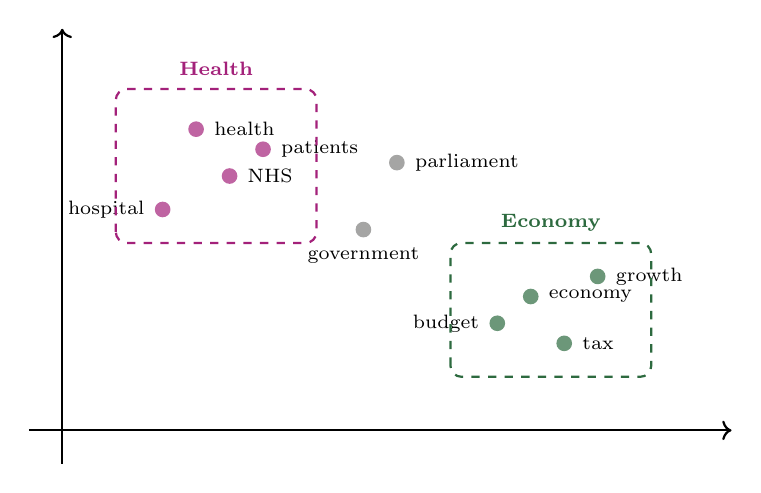
\begin{tikzpicture}[scale=0.85]
        % Axes
        \draw[thick, ->] (-0.5,0) -- (10,0);
        \draw[thick, ->] (0,-0.5) -- (0,6);

        % Health cluster
        \node[circle, fill=sgsssMagenta!70, inner sep=2pt, label=right:{\scriptsize health}] at (2,4.5) {};
        \node[circle, fill=sgsssMagenta!70, inner sep=2pt, label=right:{\scriptsize NHS}] at (2.5,3.8) {};
        \node[circle, fill=sgsssMagenta!70, inner sep=2pt, label=left:{\scriptsize hospital}] at (1.5,3.3) {};
        \node[circle, fill=sgsssMagenta!70, inner sep=2pt, label=right:{\scriptsize patients}] at (3,4.2) {};

        % Economy cluster
        \node[circle, fill=sgsssGreen!70, inner sep=2pt, label=right:{\scriptsize economy}] at (7,2) {};
        \node[circle, fill=sgsssGreen!70, inner sep=2pt, label=right:{\scriptsize tax}] at (7.5,1.3) {};
        \node[circle, fill=sgsssGreen!70, inner sep=2pt, label=left:{\scriptsize budget}] at (6.5,1.6) {};
        \node[circle, fill=sgsssGreen!70, inner sep=2pt, label=right:{\scriptsize growth}] at (8,2.3) {};

        % General words
        \node[circle, fill=sgsssBlack!40, inner sep=2pt, label=right:{\scriptsize parliament}] at (5,4) {};
        \node[circle, fill=sgsssBlack!40, inner sep=2pt, label=below:{\scriptsize government}] at (4.5,3) {};

        % Cluster outlines
        \draw[dashed, sgsssMagenta, thick, rounded corners] (0.8,2.8) rectangle (3.8,5.1);
        \node[font=\scriptsize\bfseries, text=sgsssMagenta] at (2.3,5.4) {Health};

        \draw[dashed, sgsssGreen, thick, rounded corners] (5.8,0.8) rectangle (8.8,2.8);
        \node[font=\scriptsize\bfseries, text=sgsssGreen] at (7.3,3.1) {Economy};
    \end{tikzpicture}
    \end{center}

    {\footnotesize In reality, embeddings have hundreds of dimensions. The key idea: \textbf{distance} between points captures \textbf{similarity} in meaning.}
\end{frame}

% -------------------------------------------------------
% Slide 4: What are LLMs?
% -------------------------------------------------------
\begin{frame}{What Are LLMs?}
    \begin{block}{Definition}
        \textbf{Large Language Models} are transformer-based neural networks trained on billions of words. They represent \textit{generative AI}: models that can produce new, coherent text.
    \end{block}

    \begin{columns}[T]
        \begin{column}{0.48\textwidth}
            \textbf{\color{sgsssMagenta} Proprietary (API access)}
            \begin{itemize}\setlength\itemsep{0pt}
                \item \faIcon{cloud} GPT-4 (OpenAI)
                \item \faIcon{cloud} Claude (Anthropic)
                \item \faIcon{cloud} Gemini (Google)
            \end{itemize}
            {\footnotesize Pay per use; hosted remotely; no model weights shared.}
        \end{column}
        \begin{column}{0.48\textwidth}
            \textbf{\color{sgsssGreen} Open-weight (run locally)}
            \begin{itemize}\setlength\itemsep{0pt}
                \item \faIcon{download} Llama (Meta)
                \item \faIcon{download} Mistral
                \item \faIcon{download} Qwen (Alibaba)
            \end{itemize}
            {\footnotesize Free to download; run on your own hardware; full control.}
        \end{column}
    \end{columns}

    \vspace{0.2cm}
    {\small \faIcon{info-circle} For research: choice depends on \textbf{budget}, \textbf{data sensitivity}, and \textbf{reproducibility} needs.}
\end{frame}

% -------------------------------------------------------
% Slide 3: LLMs as text analysis tools
% -------------------------------------------------------
\begin{frame}{What Can LLMs Do?}
    \small
    \begin{exampleblock}{\faIcon{tags} (a) Zero-shot classification}
        Classify text \textbf{without any training data} --- just describe the categories in a prompt.\\
        {\footnotesize \textit{Example:} ``Classify this tweet as positive, negative, or neutral.''}
    \end{exampleblock}

    \begin{exampleblock}{\faIcon{compress-alt} (b) Summarisation}
        Condense long documents into concise summaries while preserving key information.\\
        {\footnotesize \textit{Example:} ``Summarise this parliamentary debate in three bullet points.''}
    \end{exampleblock}

    \begin{exampleblock}{\faIcon{highlighter} (c) Annotation / coding}
        Apply a structured \textbf{coding scheme} to text, replicating manual qualitative coding.\\
        {\footnotesize \textit{Example:} ``Code this paragraph for policy frames: economic, moral, or rights-based.''}
    \end{exampleblock}
\end{frame}

% -------------------------------------------------------
% Slide 4: Prompt engineering for research
% -------------------------------------------------------
\begin{frame}[fragile]{Prompt Engineering for Research}
    \small
    \textbf{Key principles:}
    \begin{itemize}\setlength\itemsep{0pt}
        \item \faIcon{bullseye} \textbf{Be specific} --- define the task, audience, and expected output
        \item \faIcon{book} \textbf{Provide context} --- include background information and definitions
        \item \faIcon{list-ol} \textbf{Use examples} (few-shot) --- show input--output pairs
        \item \faIcon{code} \textbf{Request structured output} --- ask for JSON, CSV, or tables
    \end{itemize}

    \vspace{0.1cm}
    \begin{columns}[T]
        \begin{column}{0.47\textwidth}
            \begin{alertblock}{Vague prompt}
                \footnotesize
\begin{verbatim}
What is this text about?
\end{verbatim}
            \end{alertblock}
        \end{column}
        \begin{column}{0.47\textwidth}
            \begin{block}{Effective prompt}
                \footnotesize
\begin{verbatim}
Classify this text as: economy,
health, or security. Return JSON:
{"label": "...", "conf": "..."}
\end{verbatim}
            \end{block}
        \end{column}
    \end{columns}
\end{frame}

% -------------------------------------------------------
% Slide 5: Strengths and limitations
% -------------------------------------------------------
\begin{frame}{Strengths and Limitations}
    \small
    \vspace{-0.1cm}
    \begin{columns}[T]
        \begin{column}{0.48\textwidth}
            \textbf{\color{sgsssGreen} Strengths}
            \begin{itemize}\setlength\itemsep{0pt}
                \item \faIcon{magic} \textbf{Flexible} --- adapt via prompts
                \item \faIcon{ban} \textbf{No training data} --- zero/few-shot
                \item \faIcon{brain} \textbf{Handles nuance} --- context, irony
                \item \faIcon{globe} \textbf{Multilingual} --- many languages
            \end{itemize}
        \end{column}
        \begin{column}{0.48\textwidth}
            \textbf{\color{sgsssMagenta} Limitations}
            \begin{itemize}\setlength\itemsep{0pt}
                \item \faIcon{pound-sign} \textbf{Cost} --- API calls add up
                \item \faIcon{dice} \textbf{Reproducibility} --- stochastic
                \item \faIcon{exclamation-triangle} \textbf{Hallucination} --- confident but wrong
                \item \faIcon{lock} \textbf{Black box} --- hard to explain
                \item \faIcon{ruler-horizontal} \textbf{Context limits} --- finite window
            \end{itemize}
        \end{column}
    \end{columns}

    \vspace{0.15cm}
    \begin{alertblock}{Bottom line}
        LLMs are powerful but require \textbf{careful validation} against human judgements --- especially for high-stakes research.
    \end{alertblock}
\end{frame}

% -------------------------------------------------------
% Slide 6: Comparing LLMs to traditional methods
% -------------------------------------------------------
\begin{frame}{Comparing LLMs to Traditional Methods}
    \footnotesize
    \begin{center}
        \begin{tabular}{@{}l>{\raggedright\arraybackslash}p{2.2cm}>{\raggedright\arraybackslash}p{2cm}>{\raggedright\arraybackslash}p{2.3cm}>{\raggedright\arraybackslash}p{2.3cm}@{}}
            \toprule
            & \textbf{Dictionary} & \textbf{Topic models} & \textbf{Supervised} & \textbf{LLMs} \\
            \midrule
            \textbf{Training data}  & None (lexicon) & None            & Large labelled set & None (zero-shot) \\
            \textbf{Setup effort}   & Low            & Medium          & High               & Low--medium \\
            \textbf{Nuance}         & Low            & Medium          & High               & High \\
            \textbf{Reproducibility}& Perfect        & Variable        & High               & Low (stochastic) \\
            \textbf{Cost at scale}  & Negligible     & Moderate        & Low (post-train)   & High (API) \\
            \bottomrule
        \end{tabular}
    \end{center}

    \vspace{0.2cm}
    \begin{alertblock}{Key message}
        LLMs \textbf{complement} traditional methods --- they do not replace them. Use the right tool for the right task, and \textbf{validate} across approaches.
    \end{alertblock}
\end{frame}

% -------------------------------------------------------
% Slide 7: Next up
% -------------------------------------------------------
\begin{frame}{Next Up}
    \begin{center}
        {\Large \alert{Practical 4: LLM-Assisted Text Analysis}}\\[0.5cm]
        \begin{itemize}
            \item Use an LLM API to classify text at scale
            \item Experiment with prompt design and few-shot examples
            \item Compare LLM annotations with human-coded labels
            \item Discuss reproducibility and validation strategies
        \end{itemize}
        \vspace{0.5cm}
        {\normalsize Open the \textbf{Practical 4} notebook in Google Colab\\(Python or R --- your choice!)}
    \end{center}
\end{frame}

\end{document}
